\section{Derivada de Funções Paramétricas}
\subsection{Definição}
\begin{frame}
  \frametitle{Derivadas de Funções Paramétricas}
  \begin{columns}[onlytextwidth]
    \begin{column}{0.5\textwidth}\vspace{-0.5cm}
      \begin{itemize}
        \item Em \textbf{Geometria Analítica}, foram consideradas as equações paramétricas da reta
        \item De \emph{maneira geral}, podemos ter uma curva plana $\gamma$ definida por meio de equações paramétricas
        \begin{equation*}
          \gamma: \begin{cases}
            x = x(t) \\ y = y(t)
          \end{cases}\!\!\!\!\!\!\!,\,\,\,t\in [a,\,b]
        \end{equation*}
        \item Se $x(t)$ e $y(t)$ forem diferenciáveis para $t\in\, ]a,\,b[$ e $x^{\prime}(t)\not=0$, temos
        \begin{equation*}
          \frac{dy}{dx} = \frac{dy}{dt}\frac{dt}{dx} = y^{\prime}\frac{dt}{dx}
        \end{equation*}
      \end{itemize}
    \end{column}
    \begin{column}{0.5\textwidth}\vspace{-0.5cm}
      \begin{itemize}
        \item Pelo Teorema da Função Inversa, temos que
        \begin{equation*}
          \frac{dt}{dx} = \frac{1}{\dfrac{dx}{dt}} = \frac{1}{x^{\prime}(t)}
        \end{equation*}
        \item Assim, podemos escrever
        \begin{equation*}
          \frac{dy}{dx} = \frac{y^{\prime}(t)}{x^{\prime}(t)}
        \end{equation*}
        \item Observe que se $x^{\prime}(t_{0}) = 0$ em algum dado $t_{0}$, então não existirá $\dfrac{dy}{dx}(t_{0})$
      \end{itemize}
    \end{column}
  \end{columns}
\end{frame}

% \subsection{Exemplo 3}
\begin{frame}
  \begin{columns}[onlytextwidth]
    \column{0.5\textwidth}\vspace{-15pt}
      \begin{example}%{Exemplo 3}
        Considere a reta $r$ definida por \begin{equation*}
          r: \begin{cases}
            x = 2t + 1 \\ y = 4t + 3
          \end{cases}\!\!\!\!\!\!\!,\,\,\,t\in\mathbb{R}.
        \end{equation*}
        Determine a sua derivada.
      \end{example}
    \hfill
    \column{0.35\textwidth}%\vspace{-0.75cm}
  \end{columns}
\end{frame}

\subsection{Exemplo 4}
\begin{frame}
  \begin{columns}[onlytextwidth]
    \column{0.53\textwidth}\vspace{-15pt}
      \begin{example}%{Exemplo 4}
        Considere a elipse $E$ definida por \begin{equation*}
          E: \begin{cases}
            x = 4\cos{t} \\ y = 3\sen{t}
          \end{cases}\!\!\!\!\!\!\!,\,\,\,t\in[0,2\pi].
        \end{equation*}
        Determine a sua derivada, faça a \mbox{representação} gráfica e identifique os pontos em que a \mbox{equação} da elipse não é derivável.
      \end{example}
    \hfill
    \column{0.45\textwidth}%\vspace{0.25cm}
      % \begin{figure}
        % \includegraphics<1>[width=\textwidth]{figuras/fig5-0.pdf}
        % \includegraphics<2>[width=\textwidth]{figuras/fig5.pdf}
      % \end{figure}
      % \begin{itemize}
          % \item<only@+>[]\input{derivada-de-funcoes-parametricas/figuras/grid.tex}
          % \item<only@+->[]\begin{figure}[H]
    \centering
    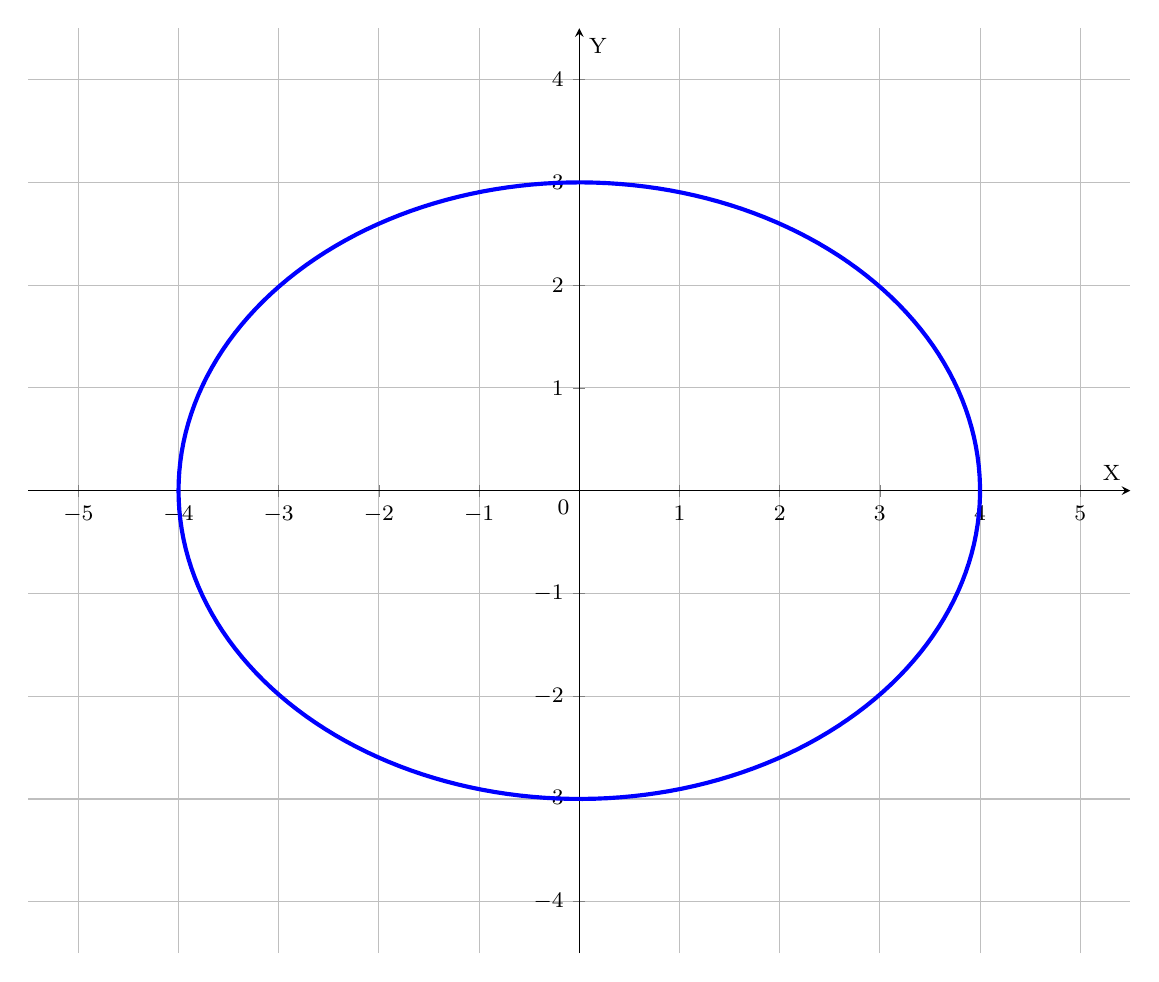
\begin{tikzpicture}
    \begin{axis}[scale=1.5,
            font=\footnotesize,
    	    width=.9\linewidth,
    		xlabel={X},ylabel={Y},
    		xtick = {-5,-4,...,5},
    		ytick = {-4,-3,...,4},
    		xmin=-5.5,xmax=5.5,
    		ymin=-4.5,ymax=4.5,
    		restrict y to domain=-5:5,
    		axis lines=center,
    		grid=both,
    		% grid style={line width=.1pt, draw=gray!10},
      %       major grid style={line width=.2pt,draw=gray!50},
      %       minor tick num=4,enlargelimits={abs=0.5},
    		% axis lines=center,
    % 		axis equal image,
    		]
    		
    		\node[below left] at (0,0) {$0$};
        	
        	\addplot[domain=-pi:pi,samples=200,
line width=1.5pt, blue] ({4*cos(deg(x))},{3*sin(deg(x))});
        	% \addplot[only marks,mark =*,blue,line width=2.5pt] coordinates{(-2,2) (10,2) (4,-2) (4,6)};
    	\end{axis}    
    \end{tikzpicture}
    % \caption{Caption}
    % \label{fig:my_label}
\end{figure}
          \only<1>{\input{derivada-de-funcoes-parametricas/figuras/grid.tex}}
          \only<2>{\begin{figure}[H]
    \centering
    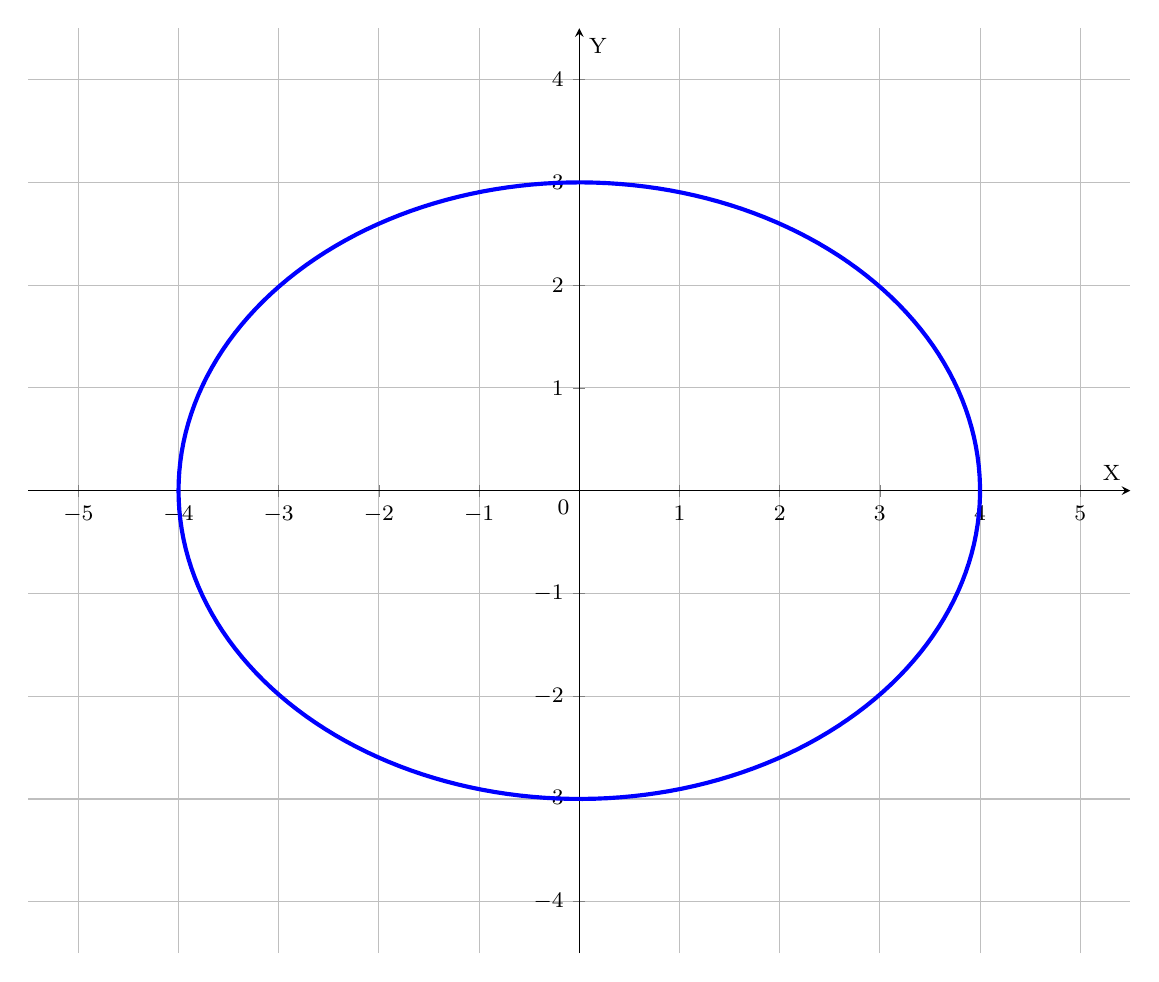
\begin{tikzpicture}
    \begin{axis}[scale=1.5,
            font=\footnotesize,
    	    width=.9\linewidth,
    		xlabel={X},ylabel={Y},
    		xtick = {-5,-4,...,5},
    		ytick = {-4,-3,...,4},
    		xmin=-5.5,xmax=5.5,
    		ymin=-4.5,ymax=4.5,
    		restrict y to domain=-5:5,
    		axis lines=center,
    		grid=both,
    		% grid style={line width=.1pt, draw=gray!10},
      %       major grid style={line width=.2pt,draw=gray!50},
      %       minor tick num=4,enlargelimits={abs=0.5},
    		% axis lines=center,
    % 		axis equal image,
    		]
    		
    		\node[below left] at (0,0) {$0$};
        	
        	\addplot[domain=-pi:pi,samples=200,
line width=1.5pt, blue] ({4*cos(deg(x))},{3*sin(deg(x))});
        	% \addplot[only marks,mark =*,blue,line width=2.5pt] coordinates{(-2,2) (10,2) (4,-2) (4,6)};
    	\end{axis}    
    \end{tikzpicture}
    % \caption{Caption}
    % \label{fig:my_label}
\end{figure}}
      % \end{itemize}
  \end{columns}
\end{frame}